\documentclass[12pt]{article}
\usepackage[a4paper,margin=2.54cm]{geometry}
\usepackage{graphicx}
\usepackage{mathptmx}
\usepackage{setspace}
\setlength{\parindent}{0pt}
\setlength{\parskip}{1em}
\begin{document}
\begin{center}\textbf{\large Supplementary Material}\\[4pt]A Cost-Matched Benchmark of Adaptive Modality Acquisition for Alzheimer's Disease Prognosis on ADNI\end{center}

Supplementary figures referred to in the main text. All figures use the 12-measure MRI block and the 24-month benchmark unless stated.

\begin{figure}[!htbp]
\centering
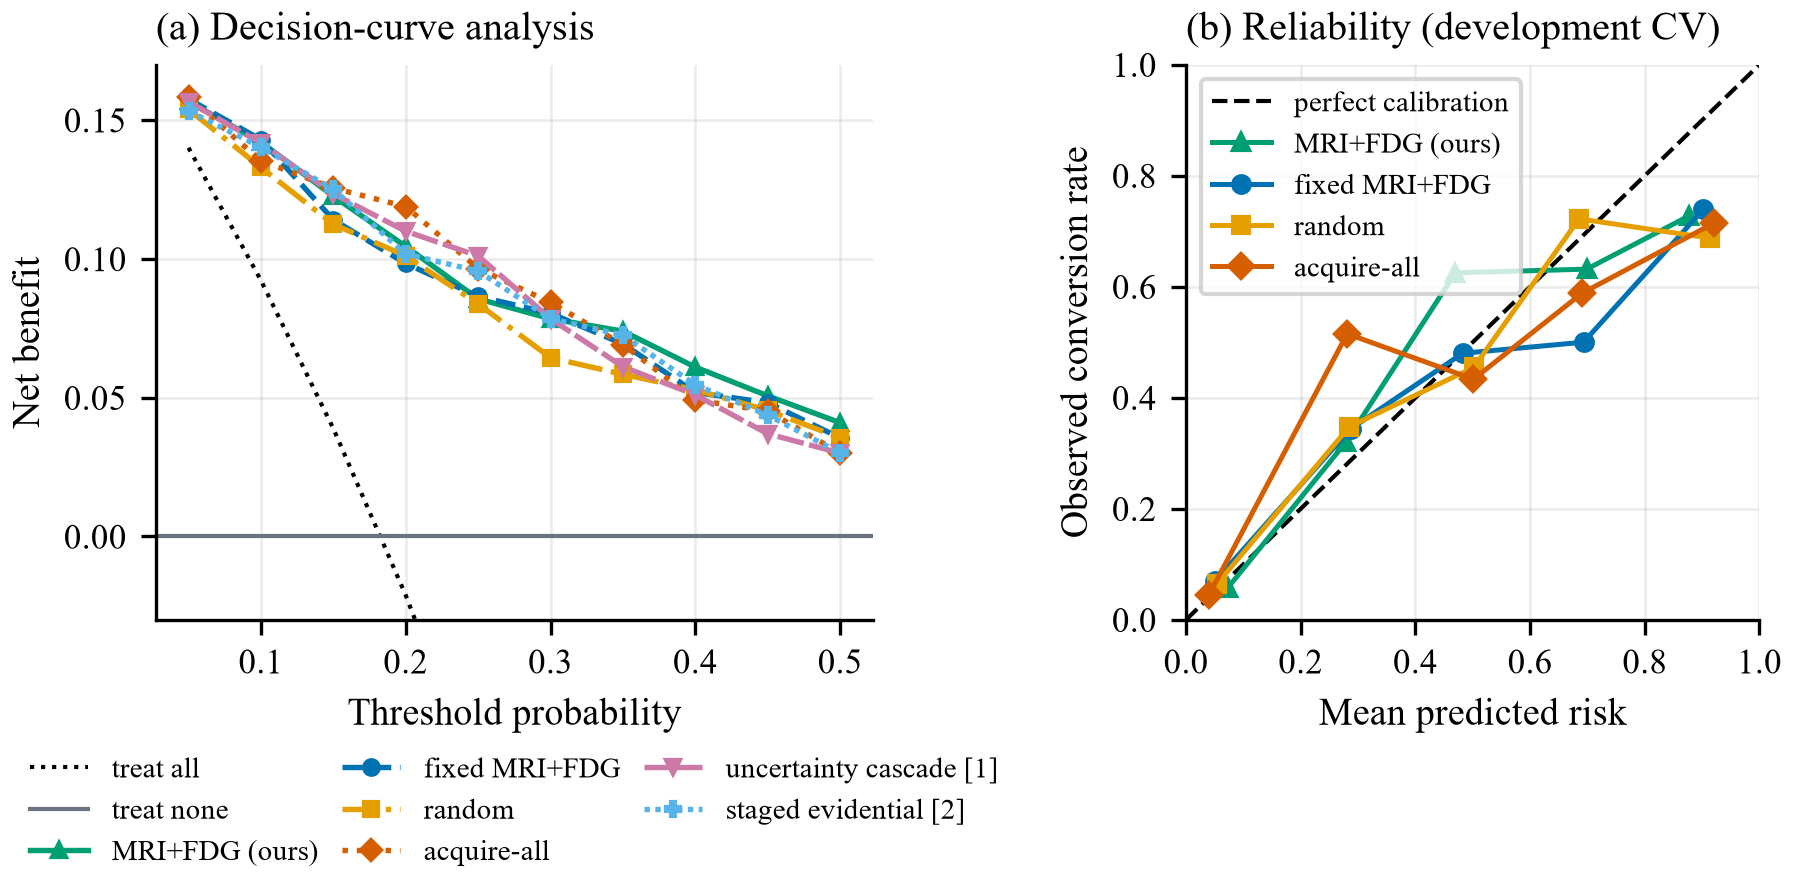
\includegraphics[width=\textwidth]{fig6_clinical_utility.png}
\par\vspace{3pt}
\textbf{Figure S1.} (a) Net benefit across threshold probabilities in the
24-month benchmark, with treat-all and treat-none references (RL policy not
shown, for legibility). (b) Reliability diagram: mean predicted risk against
observed conversion rate within risk bins.
\end{figure}

\begin{figure}[!htbp]
\centering
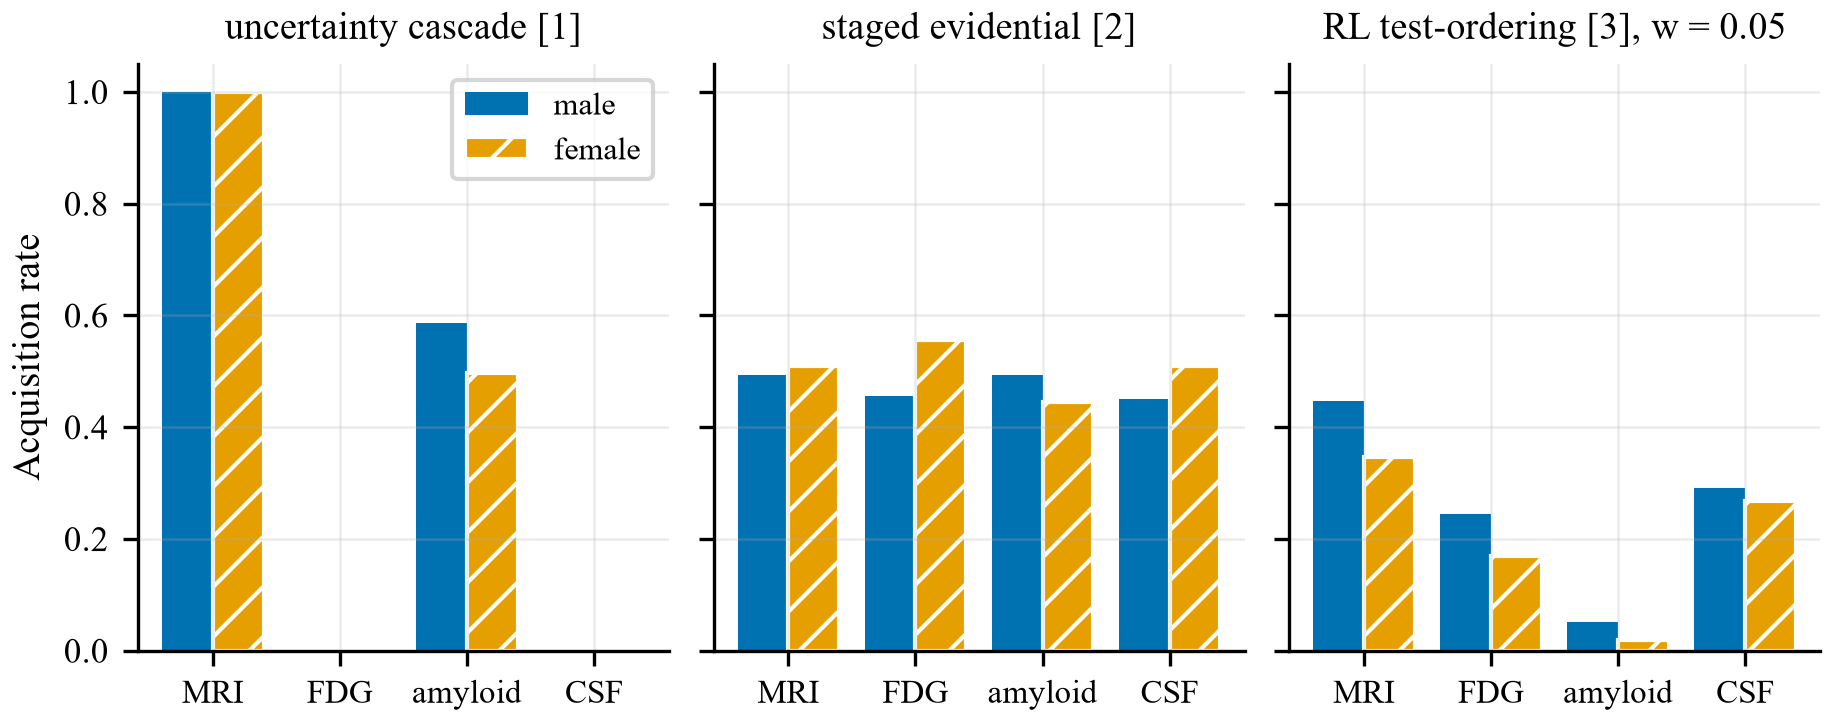
\includegraphics[width=\textwidth]{fig_sex_acquisition.png}
\par\vspace{5pt}
\textbf{Figure S2.} Acquisition rate by modality and sex for the three
published policies at 24 months (RL policy at cost weight 0.05; male $n=213$,
female $n=153$). No gap survived Benjamini-Hochberg correction.
\vspace{10pt}
\end{figure}

\begin{figure}[!htbp]
\centering
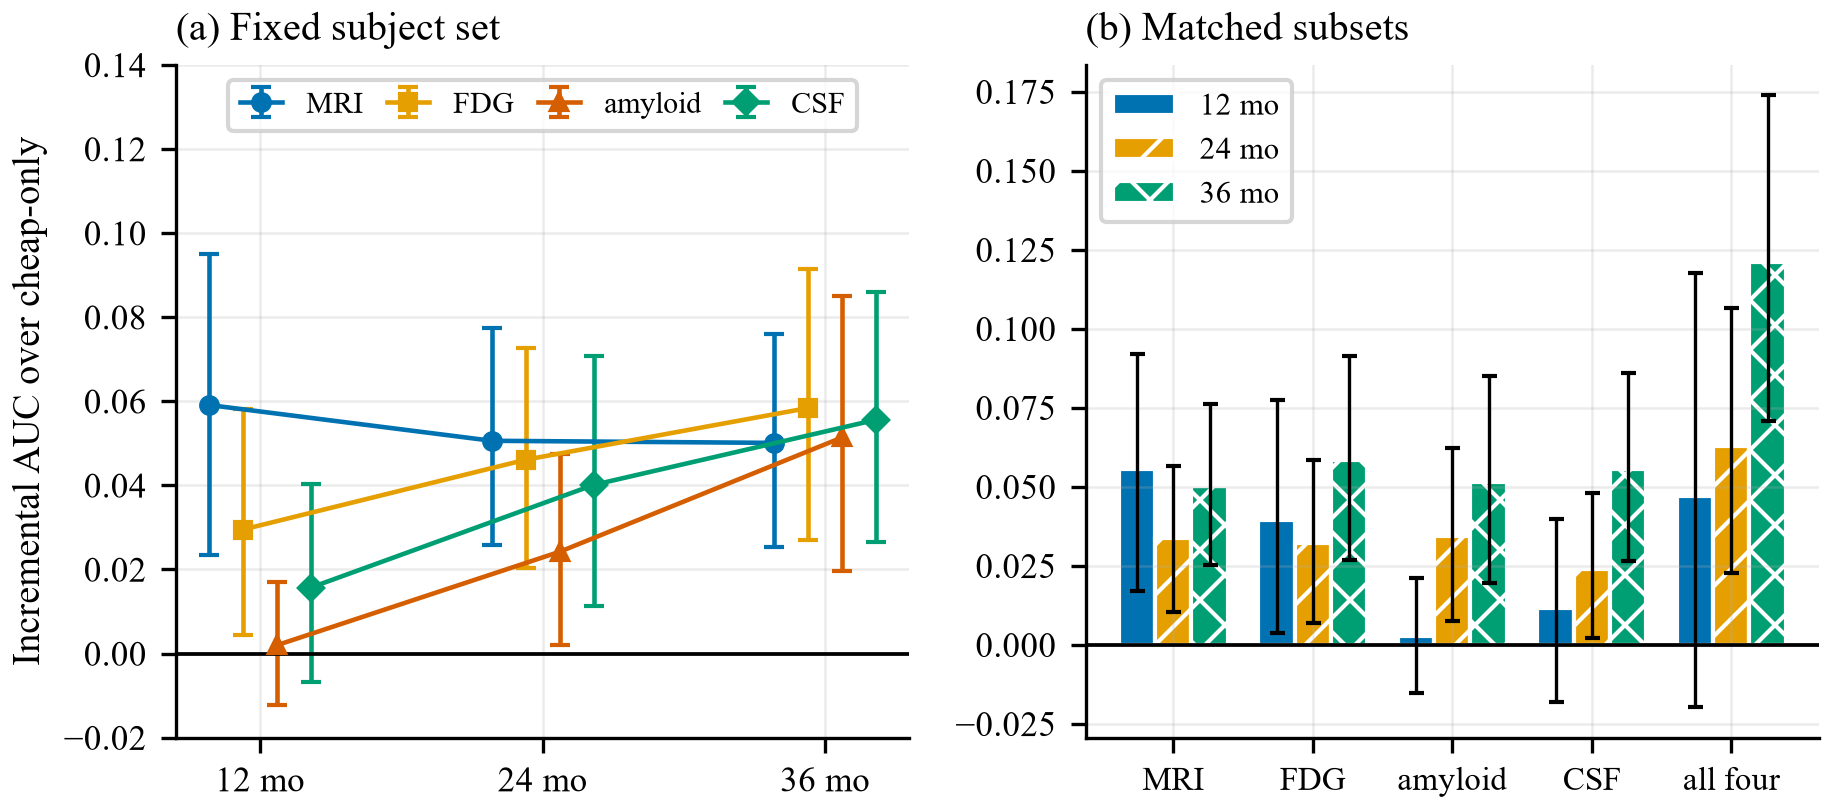
\includegraphics[width=\textwidth]{fig11_horizon.png}
\par\vspace{3pt}
\textbf{Figure S3.} (a) Incremental AUC of each modality over the cheap-only model at 12, 24 and 36 months on a fixed subject set (95\% CI); tau-PET omitted as underpowered. (b) The same quantity on subjects matched to each modality; the
all-four estimate rises from +0.047 at 12 months to +0.121 at 36 months. Both
panels use the 12-measure MRI block.
\end{figure}

\begin{figure}[!htbp]
\centering
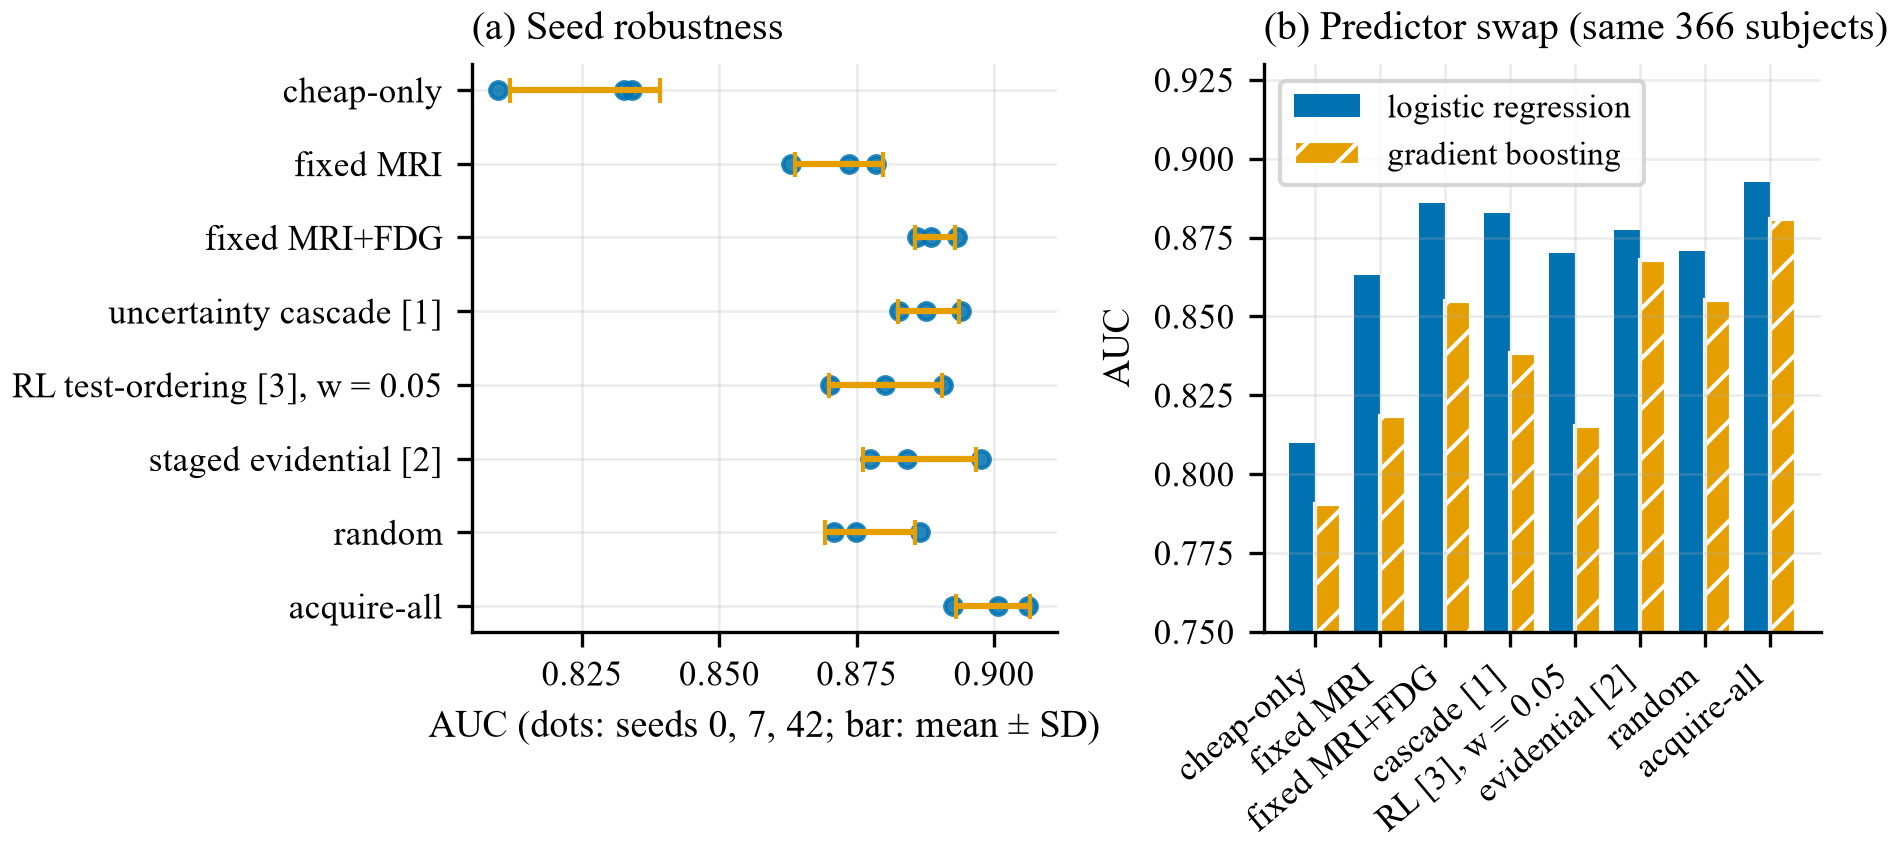
\includegraphics[width=\textwidth]{fig5_robustness.png}
\par\vspace{3pt}
\textbf{Figure S4.} (a) Seed robustness at 24 months: dots are seeds 0, 7
and 42; the bar is mean $\pm$ SD. (b) AUC under the shared logistic
regression and under gradient boosting on the same 366-subject cohort (seed
42). Both panels use the 12-measure MRI block.
\end{figure}

\begin{figure}[!htbp]
\centering
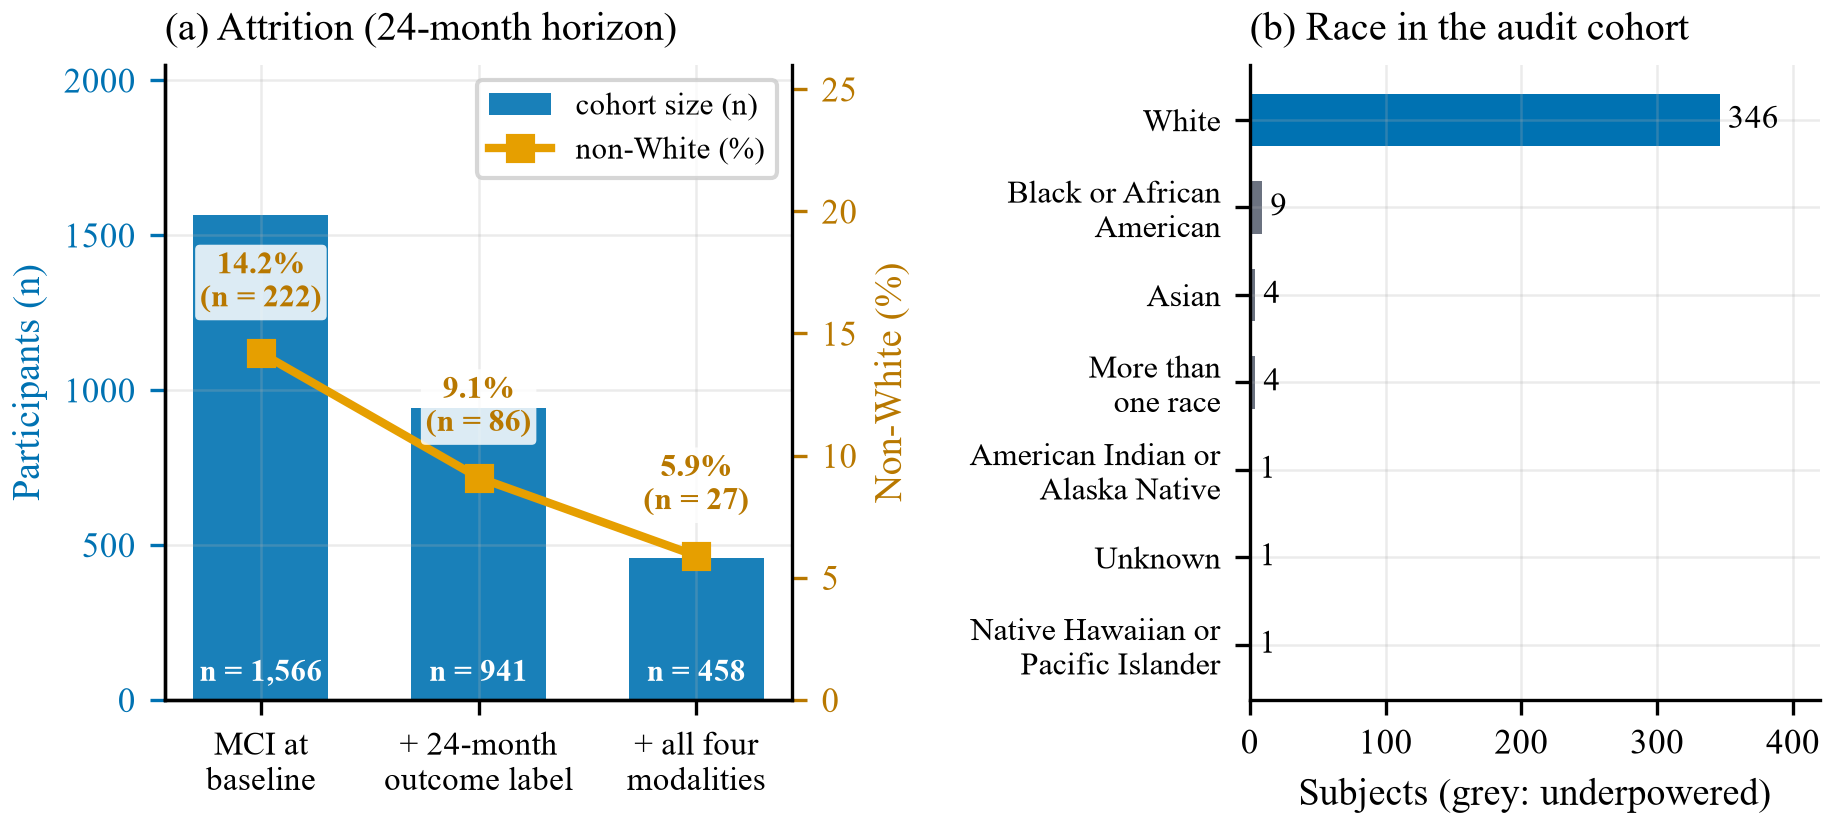
\includegraphics[width=\textwidth]{fig9_attrition.png}
\par\vspace{3pt}
\textbf{Figure S5.} (a) Cohort size (blue bars, left axis) and non-White representation (orange line, right axis) at each stage of complete-case cohort construction, 24 months. (b) Participants by self-reported race in the 24-month audit cohort; grey bars mark groups too small for stratified inference.
\end{figure}

\end{document}
